\section{Lasso Regression}
So far we have considered:
\[
    \underline{y} = X\underline{w} \hspace{1cm} X \in \mathbb{R}^{n \times p} \text{ and } \begin{Bmatrix}
        \text{Least Squares}: \underline{\hat{w}}_LS\\
        \text{Ridge Regression}: \underline{\hat{w}}_{RR}\\
    \end{Bmatrix} \underline{w} \in \mathbb{R}^p \text{ dense vector, i.e. not many zeros} 
\]
We are going to see a method which obtain a vector $\underline{\hat{w}}$ with many zeros, as sparse as possible. We want to consider this model:
\[
    \underline{y} = X\underline{w} \hspace{1cm} X \in \mathbb{R}^{n \times p} \hspace{1cm} p > n 
\]
We have said that the system is undetermined since it has infinite solutions. Suppose to have 2 features and 1 sample. 
\[
    X = \begin{bmatrix}
        2 & 3\\
    \end{bmatrix}
    \hspace{1cm}
    y = \begin{bmatrix}
        1\\
    \end{bmatrix}
\]
And so:
\[
    1 = \begin{bmatrix}
        2 & 3
    \end{bmatrix}\begin{bmatrix}
        w_1\\
        w_2
    \end{bmatrix} \implies
    1 = 2w_1 + 3w_2 \hspace{0.2cm} \leftarrow \hspace{0.2cm} \text{line}    
\]
As mentioned in a previous lecture, we want to find the minimum length solution so we can plot the line found before and the circles that represents the l2-norm distance.
\begin{center}
    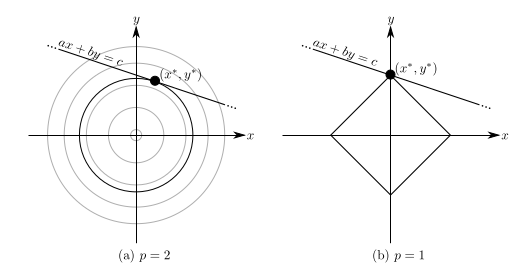
\includegraphics[scale=0.6]{../images/LassoRidgePlot.png}
\end{center}
On the right-hand side it is represented the equivalent plot but with the l1-norm. We can see that the solution on the right has one coordinate (are features!) that is equal to zero. This is true in general, i.e. we will obtain sparser solution using the l1-norm rather than the l2-norm.\\
With L1-norm it's still a convex optimization problem and
\[
    F(\underline{w}) = ||X\underline{w} - \underline{y}||_2^2 + \lambda ||\underline{w}||_1    
\] 
This model is implemented by \textbf{Lasso} (Least Absolute Shrinkage and Selection Operator) and achieve both the shortest distance solution and the selection of some features.

This is important because by reducing the number of features, we increase the interpretability of the model.\\

There is also the \textbf{Elastic Net} which combines both Lasso and Ridge: 
\[
    F(\underline{w}) = ||X\underline{w} - \underline{y}||_2^2 + \lambda_1||\underline{w}||_1 + \lambda_2||\underline{w}||_2^2  
\] 
\newpage
\section{Kernel Methods}

Kernel methods extend linear models to capture non-linear relationships without explicitly computing high-dimensional feature representations.

\subsection*{Feature Maps}

We start by transforming our original feature vector $x_\underline{x}$ using a feature map $\phi(x)$:
\[
    \phi(x) = \begin{bmatrix}
        x_1 \\ x_2 \\ x_1^2 \\ x_2^2 \\ x_1x_2
    \end{bmatrix} \in \mathbb{R}^d \quad (d > p \text{ typically})
\]

This leads to a new model representation:
\[
    \hat{y}_i = \phi(x_i)^\intercal \underline{w}
\]

\subsection*{The Kernel Trick}

To avoid computing large vectors, we introduce the kernel trick:
\[
    K(\underline{x}_i, \underline{x}_j) = \phi(\underline{x}_i)^\intercal \phi(\underline{x}_j)
\]

Common kernel functions include:
\begin{itemize}
    \item Polynomial of degree $q$: $K(\underline{x}_i, \underline{x}_j) = (\underline{x}_i^\intercal \underline{x}_j)^q$
    \item Polynomial of degree up to $q$: $K(\underline{x}_i, \underline{x}_j) = (\underline{x}_i^\intercal \underline{x}_j + 1)^q$
    \item Gaussian RBF: $K(\underline{x}_i, \underline{x}_j) = \exp(-\frac{||\underline{x}_i - \underline{x}_j||_2^2}{2\sigma^2})$
\end{itemize}

\subsection*{Kernel Ridge Regression}

In kernel ridge regression, we compute:
\[
    \underline{\alpha} = (K + \lambda I)^{-1} \underline{y}
\]
The matrix $K$ associated to Kernel has entries
\[ K_{i,j} = K(x_i, x_j) = \Phi(x_i)^T \Phi(x_j) \]

\[ \alpha = (\Phi^T \Phi + \lambda I)^{-1}  y = (K + \lambda I)^{-1} y \]

\[ y = w^T \Phi(x) = (\Phi^T \alpha)^T \Phi(x) = \alpha^T \Phi(x) \]
\[ = \sum_{i=1}^n \alpha_i (\Phi(x_i)^T \Phi(x)) \]
\[ = \sum_{i=1}^n \alpha_i K(x, x_i) \] % how far is the new sample from x_i

% contribution of sample i to the definition of decision boundary

\textbf{NB} notice that in this way, $\alpha$ can be computed without the feature map (costly), but only using the Kernel function (cheap!). 
$K$ could be singular, the term $\lambda I$ avoids the singular case
This technique is called \textit{Kernel trick}.


\subsection*{Representer Theorem}

Let $\hat{y}_i = w^T \Phi(x_i)$ with fixed feature map $\Phi$ and $w$ is learned from data $\{x_i, y_i\}$. Furthermore, let $L(y, \hat{y})$ be any loss function and $h: [0, +\infty) \rightarrow \mathbb{R}$ a strictly monotonically increasing function. Then each minimizer $w$ of
\[ \frac{1}{n} \sum_{i=1}^n L(y_i, w^T \Phi(x_i)) + h(\|w\|^2) \] % L2 regularization term
can be written as $w = \Phi^T \alpha$, where $\alpha$ is $n$-dimensional.

\textbf{NB:} A \textit{loss function} is a function that maps a single sample to a real number
\[ L(\phi, \hat{y}(x_i)) \]
then the \textit{cost function} concerns the entire sample set
\[ \frac{1}{n} \sum_{i=1}^n L(y_i, \hat{y}(x_i)) \]

\subsection*{Support Vector Regression}

Support Vector Regression (SVR) employs an $\epsilon$-insensitive loss function, which ignores errors within a certain threshold $\epsilon$. The loss function is defined as:
\[ 
L(y_i, \hat{y}) = \max(0, |y_i - \hat{y}| - \epsilon) 
\]
\[ 
= \begin{cases} 
0 & \text{if } |y_i - \hat{y}| \leq \epsilon, \\
|y_i - \hat{y}| - \epsilon & \text{otherwise.}
\end{cases} 
\]
Here, $\epsilon$ is a user-defined parameter that sets the width of the tube within which no penalty is given for errors.

The objective in SVR is to find the weight vector $w$ that minimizes the following primal formulation:
\[ 
\hat{w} = \arg\min_w \left\{ \frac{1}{n} \sum_{i=1}^n \max(0, |y_i - w^T \Phi(x_i)| - \epsilon) + \lambda \|w\|^2 \right\} 
\]
This formulation includes an $L_2$ regularization term controlled by $\lambda$, which helps prevent overfitting by penalizing the magnitude of the coefficients.

Although a direct dual formulation similar to the linear case is challenging to derive in the non-linear scenario, the dual problem in SVR can be formulated using kernel functions. The predicted value $\hat{y}(x)$ using the dual coefficients is expressed as:
\[ 
\hat{y}(\tilde{x}) = \hat{\alpha}^T K(X, \tilde{x}) 
\]
Where $K$ is the kernel function, encapsulating the inner product of vectors in a transformed feature space.

The dual coefficients $\alpha$ are obtained by solving:
\[ 
\hat{\alpha} = \arg\min_{\alpha} \frac{1}{2} \alpha^T K(X, X) \alpha - \alpha^T y + \epsilon \| \alpha \|_1 
\]
subject to the constraint $|\alpha_i| \leq \frac{1}{2n\lambda}$, which ensures that the solution does not overfit and that the influence of each data point is limited.



